\documentclass{article}


% if you need to pass options to natbib, use, e.g.:
%     \PassOptionsToPackage{numbers, compress}{natbib}
% before loading neurips_2023


% ready for submission
\usepackage[final]{neurips_2023}


% to compile a preprint version, e.g., for submission to arXiv, add add the
% [preprint] option:
%     \usepackage[preprint]{neurips_2023}


% to compile a camera-ready version, add the [final] option, e.g.:
%     \usepackage[final]{neurips_2023}


% to avoid loading the natbib package, add option nonatbib:
%    \usepackage[nonatbib]{neurips_2023}

\usepackage[utf8]{inputenc} % allow utf-8 input
\usepackage[T1]{fontenc}    % use 8-bit T1 fonts
\usepackage{hyperref}       % hyperlinks
\usepackage{url}            % simple URL typesetting
\usepackage{booktabs}       % professional-quality tables
\usepackage{amsfonts}       % blackboard math symbols
\usepackage{amsmath}
\usepackage{nicefrac}       % compact symbols for 1/2, etc.
\usepackage{microtype}      % microtypography
\usepackage{xcolor}         % colors
\usepackage{graphicx}
\usepackage{float}
\usepackage{subfig}
\usepackage[most]{tcolorbox}
\usepackage{multicol}

\bibliographystyle{plainnat}


\title{ECEN 757 | Homework 5}


% The \author macro works with any number of authors. There are two commands
% used to separate the names and addresses of multiple authors: \And and \AND.
%
% Using \And between authors leaves it to LaTeX to determine where to break the
% lines. Using \AND forces a line break at that point. So, if LaTeX puts 3 of 4
% authors names on the first line, and the last on the second line, try using
% \AND instead of \And before the third author name.

\author{%
  Muhammed U. Ersoy\\
  M.S. ECEN Student\\
  Texas A\&M University\\
  \texttt{mue@tamu.edu} \\
 }

\begin{document}
\maketitle

\begin{tcolorbox}[colback=blue!5!white,colframe=blue!75!black,title=Question 1]
    Consider a chord system with m=7. There are 42 servers. The IDs are: 3,6,9,....,126. A file has a
        hash value of 70. Where is it stored?
    \tcblower
    The file would be stored at the first peer that is greater than or equivalent to its hash value $key (\mod 2^m) \rightarrow 70 (\mod 2^7) = 70$.
    In this case it would be stored at the first peer with id $\textbf{72}$.
\end{tcolorbox}
\begin{tcolorbox}[colback=blue!5!white,colframe=blue!75!black,title=Question 2]
    For the same above, List the finger table of node 30 and for node 15.
    \tcblower
    For node $30$:
    \begin{table}[H]
    \begin{tabular}{ll}
    i & ft{[}i{]} \\ \hline
    0 & 33        \\
    1 & 33        \\
    2 & 36        \\
    3 & 39        \\
    4 & 48        \\
    5 & 63        \\
    6 & 96       
    \end{tabular}
    \end{table}

    For node $15$:
    \begin{table}[H]
    \begin{tabular}{ll}
    i & ft{[}i{]} \\ \hline
    0 & 18        \\
    1 & 18        \\
    2 & 21        \\
    3 & 24        \\
    4 & 33        \\
    5 & 48        \\
    6 & 81       
    \end{tabular}
    \end{table}
\end{tcolorbox}

\begin{tcolorbox}[colback=blue!5!white,colframe=blue!75!black,title=Question 3]
    The following is an overlay of Gnutella. Suppose node 7 starts a query with TTL = 2. Which nodes
    receive the query? Explain your answer
    \begin{figure}[H]
        \centering
        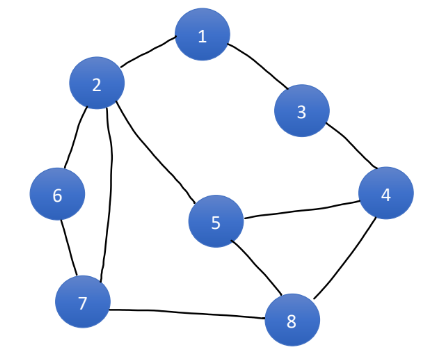
\includegraphics[width=5cm]{q3.png}
    \end{figure}
    \tcblower
    As seen in the graph below node 7 would send the query message to its immediate neighbours $\{ 2,6,8\}$(red arrows). 
    Which the receiving nodes would mark as $hop = 1$ and the header would have $ttl = 2$ since $hop < ttl$ they would
    forward the message to their immediate neighbours $2 \rightarrow \{1,5,6\}$, $6 \rightarrow \{2\}$,
    and $8 \rightarrow \{4,5\}$. These are marked by the orange arrows. In this jump $hop = 2$ and since $hop = ttl$ the flooding would terminate at this step.
    \begin{figure}[H]
        \centering
        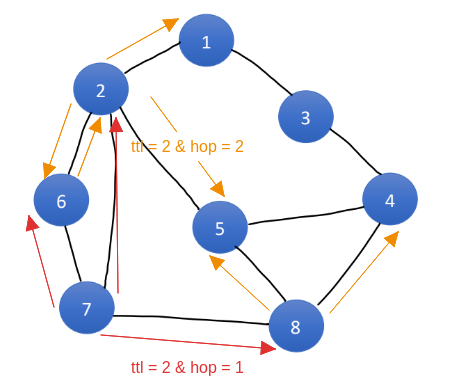
\includegraphics[width=5cm]{q3_answer.png}
    \end{figure}

\end{tcolorbox}

\begin{tcolorbox}[colback=blue!5!white,colframe=blue!75!black,title=Question 4 (10.7)]
    Explain why using the secure hash of an object to identify and route messages to it is
    tamper-proof. What properties are required of the hash function? How can integrity be
    maintained, even if a substantial proportion of peer nodes are subverted?
    \tcblower
    - The use of a secure hash makes a resource `self-certifying`. A requestor can validate the requested resource by comparing with its hash.
    This way an untrusted source cannot replace the \textit{real} resource with a fake/malicious one.\\
    - The function should be random to randomly distribute resources over the overlay network. It should not
    be a function to `place` similar objects next to each other or give them similar hashes.
    
    \begin{enumerate}(1)
        Hash functions should have a reasonable uniqueness guarantee.\\ For SHA-1 to have a $50\%$ chance
        of a hash collision, there would have to be $1.42 \times 10^{24}$ records in the table. \citet{LINSTEDT201617} 
    \end{enumerate}
    \begin{enumerate}(2)
        Hash functions should be difficult to reverse meaning given $y = hash\_fn(x)$, $x$ must be computationally
        infeasible to compute from $y$, e.g. $x = hash\_fn^{-1}(y)$. Preventing tampering and collision searching.
    \end{enumerate}
    
    Requestors can validate the resource they receive by comparing their expected hashes with the calculated hash. This way if a subverted
    node sends a bad resource the requestor can identify it and ignore it.
\end{tcolorbox}

\begin{tcolorbox}[colback=blue!5!white,colframe=blue!75!black,title=Question 5]
    Consider a Pastry system and a node of ID – 48E175. The following is snap of its routing table.
    \begin{figure}[H]
        \centering
        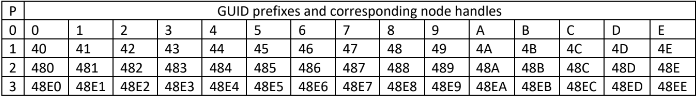
\includegraphics[scale=0.70]{q5.png}
    \end{figure}
    this node has to send packets to nodes,
    \begin{itemize}(a) 48E322
    \end{itemize}
    \begin{itemize}(b) 54A666
    \end{itemize}
    Explain how the routing takes place to send packets to the nodes given above.
\tcblower
\begin{itemize}(a) \\
    1. The first step is to look at the GUID prefix table and figure out the largest matching prefix. In this
    case it is \textcolor{red}{48E3}XX $\rightarrow n$ where n is the handle of a node matching this pattern. 
    then the current node (48E175) would route the message to $n$ which would compare the delivery id with its own. If it's not the final
    destination it would look at its' own GUID table to find a closer destination. And the process would continue until the message reaches its' final destination.
\end{itemize}
\begin{itemize}(b) \\
    Similar to the previous example the current node would first look at the ID in the message and compare to its own. Then it would look at the GUID table
and find the largest matching GUID prefix. In this case it would be \textcolor{red}{5}XXXXX $\rightarrow n$.
\end{itemize}
\end{tcolorbox}

\bibliography{default}
\end{document}


